\section{John Hendry Park (Trout Lake)}

\begin{figure}[h]
  \centering
    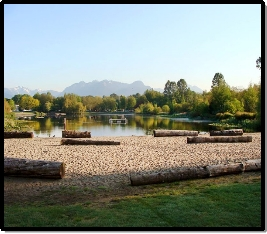
\includegraphics{tlcover.jpg}
\end{figure}

John Hendry Park is a 27 hectare park located in the heart of East Vancouver. Commonly known as Trout Lake, the body of water in the centre of the park, the park itself is named after the owner of one of Vancouver’s first lumber mills, which was located in the park. 

Easily accessed from Commercial Drive, Nanaimo St, or East 12th Ave, it is a popular location for birders and nature-lovers alike in the Vancouver area. The park is also home to the Trout Lake Community Centre which provides many services to the local community. Over 135 species of birds have been observed at Trout Lake, including seven species of conservation concern. The park reaches its peak diversity during spring and fall migration, with the fewest number of birds and species during the summer. 

Trout Lake itself usually has a large number of Mallard and wigeon, with a few other species of ducks, plus American Coots and Pied-billed Grebes from October through April. During the same time period many gulls use the lake for bathing and drinking first thing in the morning. This park has proven notable for being one of the most reliable locations for finding California and Western Gulls during this period. 

Anna’s Hummingbirds are frequently seen on the tops of small trees surrounding the lake.
